%-----------------------------------
% Define document and include general packages
%-----------------------------------
% Tabellen- und Abkürzungsverzeichnis stehen normalerweise nicht im
% Inhaltsverzeichnis. Gleiches gilt für das Abkürzungsverzeichnis (siehe unten).
% Manche Dozenten bemängeln das. Die Optionen 'listof=totoc,bibliography=totoc'
% geben das Tabellen- und Abkürzungsverzeichnis im Inhaltsverzeichnis (toc=Table
% of Content) aus.
% Da es aber verschiedene Regelungen je nach Dozent geben kann, werden hier
% beide Varianten dargestellt.
\documentclass[12pt,oneside,titlepage,listof=totoc,bibliography=totoc]{scrartcl}
%\documentclass[12pt,oneside,titlepage]{scrartcl}
%Dokumentensprache
\newif\ifde
\newif\ifen

%-----------------------------------
% Meta informationen
%-----------------------------------
%-----------------------------------
% Meta Informationen zur Arbeit
%-----------------------------------

% Autor
\newcommand{\myAutor}{Semjon Alexander Bibow}

% Adresse
\newcommand{\myAdresse}{Carl-Schurz-Str. 1a \\ \> \> \> 28209 Bremen}

% Titel der Arbeit
\newcommand{\myTitel}{Methodik zur Bewertung von IT-Infrastruktur Trends}

\newcommand{\mySubTitel}{Am Beispiel von Hybrid Cloud Technologien}

% Betreuer
\newcommand{\myBetreuer}{Mark-Oliver Würtz}

% Lehrveranstaltung
\newcommand{\myLehrveranstaltung}{IT-Infrastruktur}

% Matrikelnummer
\newcommand{\myMatrikelNr}{517450}

% Ort
\newcommand{\myOrt}{Bremen}

% Datum der Abgabe
\newcommand{\myAbgabeDatum}{\today}

% Semesterzahl
\newcommand{\mySemesterZahl}{3}

% Name der Hochschule
\newcommand{\myHochschulName}{FOM Hochschule für Oekonomie \& Management}

% Standort der Hochschule
\newcommand{\myHochschulStandort}{Bremen}

% Studiengang
\newcommand{\myStudiengang}{Wirtschaftsinformatik}

% Art der Arbeit
\newcommand{\myThesisArt}{Semesterarbeit}

% Zu erlangender akademische Grad
\newcommand{\myAkademischerGrad}{Bachelor of Science (B.Sc.)}

% Firma
\newcommand{\myFirma}{CGI Deutschland B.V. & Co. KG}


\ifdefined\FOMEN
%Englisch
\entrue
\usepackage[english]{babel}
\else
%Deutsch
\detrue
\usepackage[ngerman]{babel}
\fi


\newcommand{\langde}[1]{%
   \ifde\selectlanguage{ngerman}#1\fi}
\newcommand{\langen}[1]{%
   \ifen\selectlanguage{english}#1\fi}
\langde{\usepackage[babel,german=quotes]{csquotes}}
\langen{\usepackage[babel,english=british]{csquotes}}
\usepackage[utf8]{luainputenc}
\usepackage[T1]{fontenc}
\usepackage{fancyhdr}
\usepackage{fancybox}
\usepackage[a4paper, left=4cm, right=2cm, top=4cm, bottom=2cm]{geometry}
\usepackage{graphicx}
\usepackage{wrapfig}
\usepackage{gensymb}
\usepackage{colortbl}
\usepackage[capposition=top]{floatrow}
\usepackage{array}
\usepackage{float}      %Positionierung von Abb. und Tabellen mit [H] erzwingen
\usepackage{footnote}
% Darstellung der Beschriftung von Tabellen und Abbildungen (Leitfaden S. 44)
% singlelinecheck=false: macht die Caption linksbündig (statt zentriert)
% labelfont auf fett: (Tabelle x.y:, Abbildung: x.y)
% font auf fett: eigentliche Bezeichnung der Abbildung oder Tabelle
% Fettschrift laut Leitfaden 2018 S. 45
\usepackage[singlelinecheck=false, labelfont=bf, font=bf]{caption}
\usepackage{caption}
\usepackage[colorlinks=true,linkcolor=black]{hyperref}
\usepackage{amssymb}
\usepackage{mathptmx}
%\usepackage{minted} %Kann für schöneres Syntax Highlighting genutzt werden. ACHTUNG: Python muss installiert sein.
\usepackage[scaled=0.9]{helvet} % Behebt, zusammen mit Package courier, pixelige Überschriften. Ist, zusammen mit mathptx, dem times-Package vorzuziehen. Details: https://latex-kurs.de/fragen/schriftarten/Times_New_Roman.html
\usepackage{courier}
\usepackage{amsmath}
\usepackage{enumitem,cleveref}
\usepackage[table]{xcolor}
\usepackage{marvosym}			% Verwendung von Symbolen, z.B. perfektes Eurozeichen
\definecolor{darkblack}{rgb}{0,0,0}
\hypersetup{colorlinks=true, breaklinks=true, linkcolor=darkblack, menucolor=darkblack, urlcolor=darkblack}
\renewcommand\familydefault{\sfdefault}
\usepackage{ragged2e}

% Mehrere Fussnoten nacheinander mit Komma separiert
\usepackage[hang, multiple]{footmisc}
\setlength{\footnotemargin}{1em}

% todo Aufgaben als Kommentare verfassen für verschiedene Editoren
%\usepackage{todonotes}

%Pakete für Tabellen
\usepackage{epstopdf}
\usepackage{nicefrac} % Brüche
\usepackage{multirow}
\usepackage{rotating} % vertikal schreiben
\usepackage{mdwlist}
\usepackage{tabularx}% für breitenangabe

\definecolor{dunkelgrau}{rgb}{0.8,0.8,0.8}
\definecolor{hellgrau}{rgb}{0.0,0.7,0.99}
% Colors for listings
\definecolor{mauve}{rgb}{0.58,0,0.82}
\definecolor{dkgreen}{rgb}{0,0.6,0}

% sauber formatierter Quelltext
\usepackage{listings}
% JavaScript als Sprache definieren:
\lstdefinelanguage{JavaScript}{
	keywords={break, super, case, extends, switch, catch, finally, for, const, function, try, continue, if, typeof, debugger, var, default, in, void, delete, instanceof, while, do, new, with, else, return, yield, enum, let, await},
	keywordstyle=\color{blue}\bfseries,
	ndkeywords={class, export, boolean, throw, implements, import, this, interface, package, private, protected, public, static},
	ndkeywordstyle=\color{darkgray}\bfseries,
	identifierstyle=\color{black},
	sensitive=false,
	comment=[l]{//},
	morecomment=[s]{/*}{*/},
	commentstyle=\color{purple}\ttfamily,
	stringstyle=\color{red}\ttfamily,
	morestring=[b]',
	morestring=[b]"
}

\lstset{
	%language=JavaScript,
	numbers=left,
	numberstyle=\tiny,
	numbersep=5pt,
	breaklines=true,
	showstringspaces=false,
	frame=l ,
	xleftmargin=5pt,
	xrightmargin=5pt,
	basicstyle=\ttfamily\scriptsize,
	stepnumber=1,
	keywordstyle=\color{blue},          % keyword style
	commentstyle=\color{dkgreen},       % comment style
	stringstyle=\color{mauve}         % string literal style
}

% Biblatex

\usepackage{url}
\urlstyle{same}

%%%% Neuer Leitfaden (2018)
\usepackage[
backend=biber,
style=ext-authoryear,
maxcitenames=2,	% mindestens 3 Namen ausgeben bevor et. al. kommt
maxbibnames=999,
mergedate=false,
date=iso,
seconds=true, %werden nicht verwendet, so werden aber Warnungen unterdrückt.
urldate=iso,
innamebeforetitle,
dashed=false,
autocite=footnote,
doi=false,
useprefix=true, % 'von' im Namen beachten (beim Anzeigen)
mincrossrefs = 1
]{biblatex}%iso dateformat für YYYY-MM-DD

%weitere Anpassungen für BibLaTex
\usepackage{xpatch}

\setlength\bibhang{1cm}

%%% Weitere Optionen
%\boolitem[false]{citexref} %Wenn incollection, inbook, inproceedings genutzt wird nicht den zugehörigen parent auch in Literaturverzeichnis aufnehmen

%Aufräumen die Felder werden laut Leitfaden nicht benötigt.
\AtEveryBibitem{%
\ifentrytype{book}{
    \clearfield{issn}%
    \clearfield{doi}%
    \clearfield{isbn}%
    \clearfield{url}
    \clearfield{eprint}
}{}
\ifentrytype{collection}{
  \clearfield{issn}%
  \clearfield{doi}%
  \clearfield{isbn}%
  \clearfield{url}
  \clearfield{eprint}
}{}
\ifentrytype{incollection}{
  \clearfield{issn}%
  \clearfield{doi}%
  \clearfield{isbn}%
  \clearfield{url}
  \clearfield{eprint}
}{}
\ifentrytype{article}{
  \clearfield{issn}%
  \clearfield{doi}%
  \clearfield{isbn}%
  \clearfield{url}
  \clearfield{eprint}
}{}
\ifentrytype{inproceedings}{
  \clearfield{issn}%
  \clearfield{doi}%
  \clearfield{isbn}%
  \clearfield{url}
  \clearfield{eprint}
}{}
}

\renewcommand*{\finentrypunct}{}%Kein Punkt am ende des Literaturverzeichnisses

\renewcommand*{\newunitpunct}{\addcomma\space}
\DeclareDelimFormat[bib,biblist]{nametitledelim}{\addcolon\space}
\DeclareDelimFormat{titleyeardelim}{\newunitpunct}
%Namen kursiv schreiben
\renewcommand*{\mkbibnamefamily}{\mkbibemph}
\renewcommand*{\mkbibnamegiven}{\mkbibemph}
\renewcommand*{\mkbibnamesuffix}{\mkbibemph}
\renewcommand*{\mkbibnameprefix}{\mkbibemph}

% Die Trennung mehrerer Autorennamen erfolgt durch Kommata.
% siehe Beispiele im Leitfaden S. 16
% Die folgende Zeile würde mit Semikolon trennen
%\DeclareDelimFormat{multinamedelim}{\addsemicolon\addspace}

%Delimiter für mehrere und letzten Namen gleich setzen
\DeclareDelimAlias{finalnamedelim}{multinamedelim}

\DeclareNameAlias{default}{family-given}
\DeclareNameAlias{sortname}{default}  %Nach Namen sortieren


\DeclareFieldFormat{editortype}{\mkbibparens{#1}}
\DeclareDelimFormat{editortypedelim}{\addspace}
\DeclareFieldFormat{translatortype}{\mkbibparens{#1}}
\DeclareDelimFormat{translatortypedelim}{\addspace}
\DeclareDelimFormat[bib,biblist]{innametitledelim}{\addcomma\space}

\DeclareFieldFormat*{citetitle}{#1}
\DeclareFieldFormat*{title}{#1}
\DeclareFieldFormat*{booktitle}{#1}
\DeclareFieldFormat*{journaltitle}{#1}

\xpatchbibdriver{online}
  {\usebibmacro{organization+location+date}\newunit\newblock}
  {}
  {}{}

\DeclareFieldFormat[online]{date}{\mkbibparens{#1}}
\DeclareFieldFormat{urltime}{\addspace #1\addspace \langde{Uhr}\langen{MEZ}}
\DeclareFieldFormat{urldate}{%urltime zu urldate hinzufügen
  [\langde{Zugriff}\langen{Access}\addcolon\addspace
  #1\printfield{urltime}]
}
\DeclareFieldFormat[online]{url}{<\url{#1}>}
\renewbibmacro*{url+urldate}{%
  \usebibmacro{url}%
  \ifentrytype{online}
    {\setunit*{\addspace}%
     \iffieldundef{year}
       {\printtext[date]{\langde{keine Datumsangabe}\langen{no Date}}}
       {\usebibmacro{date}}}%
    {}%
  \setunit*{\addspace}%
  \usebibmacro{urldate}
  }

%Verhindern, dass bei mehreren Quellen des gleichen Autors im gleichen Jahr
%Buchstaben nach der Jahreszahl angezeigt werden wenn sich das Keyword in usera unterscheidet.
\DeclareExtradate{
  \scope{
    \field{labelyear}
    \field{year}
    }
    \scope{
      \field{usera}
     }
}

%% Anzeige des Jahres nach dem Stichwort (usera) im Literaturverzeichnis
%% Wenn das Jahr bei Online-Quellen nicht explizit angegeben wurde, wird nach
%% dem Stichwort 'o. J.' ausgegeben. Nach der URL steht dann 'keine
%% Datumsangabe'. Ist das Jahr definiert, wird es an beiden Stellen ausgegeben.
%% Das Zugriffsdatum (urldate) spielt hier keine Rolle.
%% Für Nicht-Online-Quellen wird nichts geändert.
\renewbibmacro*{date+extradate}{%
  \printtext[parens]{%
    \printfield{usera}%
    \setunit{\printdelim{titleyeardelim}}%
    \ifentrytype{online}
       {\setunit*{\addspace\addcomma\addspace}%
         \iffieldundef{year}
           {\bibstring{nodate}}
       {\printlabeldateextra}}%
       {\printlabeldateextra}}}

%% Anzeige des Jahres nach dem Stichwort (usera) in der Fussnote
%% das Stichwort hat der Aufrufer hier schon ausgegeben.
%% siehe auch Kommentar zu: \renewbibmacro*{date+extradate}
\renewbibmacro*{cite:labeldate+extradate}{%
    \ifentrytype{online}
       {\setunit*{\addspace\addcomma\addspace}%
         \iffieldundef{year}
           {\bibstring{nodate}}
       {\printlabeldateextra}}%
       {\printlabeldateextra}}


\DefineBibliographyStrings{german}{
  nodate    = {{}o.\adddot\addspace J\adddot},
  andothers = {et\addabbrvspace al\adddot}
}
\DefineBibliographyStrings{english}{
  nodate    = {{}n.\adddot\addspace d\adddot},
  andothers = {et\addabbrvspace al\adddot}
}
\DeclareSourcemap{
  \maps[datatype=bibtex]{
    \map{
      \step[notfield=translator, final]
      \step[notfield=editor, final]
      \step[fieldset=author, fieldvalue={{{\langde{o\noexpand\adddot\addspace V\noexpand\adddot}\langen{Anon}}}}]
    }
    \map{
      \pernottype{online}
      \step[fieldset=location, fieldvalue={\langde{o\noexpand\adddot\addspace O\noexpand\adddot}\langen{s\noexpand\adddot I\noexpand\adddot}}]
    }
  }
}

\renewbibmacro*{cite}{%
  \iffieldundef{shorthand}
    {\ifthenelse{\ifnameundef{labelname}\OR\iffieldundef{labelyear}}
       {\usebibmacro{cite:label}%
        \setunit{\printdelim{nonametitledelim}}}
       {\printnames{labelname}%
        \setunit{\printdelim{nametitledelim}}}%
     \printfield{usera}%
     \setunit{\printdelim{titleyeardelim}}%
     \usebibmacro{cite:labeldate+extradate}}
    {\usebibmacro{cite:shorthand}}}

    \renewcommand*{\jourvoldelim}{\addcomma\addspace}% Trennung zwischen journalname und Volume. Sonst Space; Laut Leitfaden richtig
    \hypersetup{hidelinks} %sonst sind Fußnoten grün. Dadurch werden Links allerdings nicht mehr farbig dargestellt

\renewbibmacro*{journal+issuetitle}{%
  \usebibmacro{journal}%
  \setunit*{\jourvoldelim}%
  \iffieldundef{series}
    {}
    {\setunit*{\jourserdelim}%
     \printfield{series}%
     \setunit{\servoldelim}}%
  \iffieldundef{volume}
    {}
    {\printfield{volume}}
  \iffieldundef{labelyear}
  {}
  {
  (\thefield{year}) %Ansonsten wird wenn kein Volume angegeben ist ein Komma vorangestellt
  }
  \setunit*{\addcomma\addspace Nr\adddot\addspace}
  \printfield{number}
  \iffieldundef{eid}
  {}
  {\printfield{eid}}
}

% Postnote ist der Text in der zweiten eckigen Klammer bei einem Zitat
% wenn es keinen solchen Eintrag gibt, dann auch nicht ausgeben, z.B. 'o. S.'
% Wenn man das will, kann man das 'o. S.' ja explizit angeben. Andernfalls steht
% sonst auch bei Webseiten 'o. S.' da, was laut Leitfaden nicht ok ist.
\renewbibmacro*{postnote}{%
  \setunit{\postnotedelim}%
  \iffieldundef{postnote}
    {} %{\printtext{\langde{o.S\adddot}\langen{no page number}}}
    {\printfield{postnote}}}

% Abstand bei Änderung Anfangsbuchstabe ca. 1.5 Zeilen
\setlength{\bibinitsep}{0.75cm}

% nur in den Zitaten/Fussnoten den Vornamen abkürzen (nicht im
% Literaturverzeichnis)

\DeclareDelimFormat{nonameyeardelim}{\addcomma\space}
\DeclareDelimFormat{nameyeardelim}{\addcomma\space}

\renewbibmacro*{cite}{%
  \iffieldundef{shorthand}
    {\ifthenelse{\ifnameundef{labelname}\OR\iffieldundef{labelyear}}
       {\usebibmacro{cite:label}%
        \setunit{\printdelim{nonameyeardelim}}}
      {\toggletrue{abx@bool@giveninits}
        \printnames[family-given]{labelname}%
        \setunit{\printdelim{nameyeardelim}}}%
      \printfield{usera}%
      \setunit{\printdelim{titleyeardelim}}%
     \usebibmacro{cite:labeldate+extradate}}
   {\usebibmacro{cite:shorthand}}}


%%%%% Alter Leitfaden. Ggf. Einkommentieren und Bereich hierüber auskommentieren
%\usepackage[
%backend=biber,
%style=numeric,
%citestyle=authoryear,
%url=false,
%isbn=false,
%notetype=footonly,
%hyperref=false,
%sortlocale=de]{biblatex}

%weitere Anpassungen für BibLaTex
%% Opptionen für Biblatex
\ExecuteBibliographyOptions{%
giveninits=false,
isbn=true,
url=true,
doi=false,
eprint=false,
maxbibnames=7, % Alle Autoren (kein et al.)
maxcitenames=2, % et al. ab dem 3. Autor
backref=false, % Rückverweise auf Zitatseiten
bibencoding=utf8, % wenn .bib in utf8, sonst ascii
bibwarn=true, % Warnung bei fehlerhafter bib-Datei
}%

% et al. an Stelle von u.a.
\DefineBibliographyStrings{ngerman}{
   andothers = {{et\,al\adddot}},
}

% Klammern um das Jahr in der Fußnote
\renewbibmacro*{cite:labelyear+extrayear}{%
  \iffieldundef{labelyear}
    {}
    {\printtext[bibhyperref]{%
       \mkbibparens{%
         \printfield{labelyear}%
         \printfield{extrayear}}}}}

\renewbibmacro*{cite:title}{%
  \printtext[bibhyperref]{%
    \printfield[citetitle]{labeltitle}%
    \setunit{\addcomma\space}%
    \printdate}}

\DeclareNameFormat{last-first}{%
  \iffirstinits
    {\usebibmacro{name:family-given}
        {\namepartfamily}
        {\namepartgiveni}
        {\namepartprefix}
        {\namepartsuffix}
    }
    {\usebibmacro{name:family-given}
        {\namepartfamily}
        {\namepartgiven}
        {\namepartprefix}
        {\namepartsuffix}
    }%
  \usebibmacro{name:andothers}}

% Alternative Notation der Fußnoten
% Zeigt sowohl den Nachnamen als auch den Vornamen an
% Beispiel: \fullfootcite[Vgl. ][Seite 5]{Tanenbaum.2003}
\DeclareCiteCommand{\fullfootcite}[\mkbibfootnote]
  {\usebibmacro{prenote}}
  {\usebibmacro{citeindex}%
    \printnames[sortname][1-1]{author}%
    \addspace (\printfield{year})}
  {\addsemicolon\space}
  {\usebibmacro{postnote}}

%Autoren (Nachname, Vorname)
\DeclareNameAlias{default}{family-given}

%Reihenfolge von publisher, year, address verändern
% Achtung, bisher nur für den Typ @book definiert

%% Definiert @Book Eintrag
\DeclareBibliographyDriver{book}{%
  \printnames{author}%
  \newunit\addcolon\space
  \printfield{title}%
  \setunit*{,\space}%
  \printfield{edition}%
  \setunit*{\addcomma\space}%
  \printlist{publisher}%
  \newunit\newblockpunct
  \printlist{location}%
  \setunit*{\space}%
  \printfield{year}%
  \setunit*{,\space}%
  \printfield{isbn}%
  \finentry}

%% Definiert @Online Eintrag
\DeclareBibliographyDriver{online}{%
  \printnames{author}%
  \newunit\newblockpunct
  \printfield{title}%
  \setunit*{,\space}%
  %\newunit\newblock
  \printfield{url}%
  \setunit*{,\space Erscheinungsjahr:\space}%
  \printfield{year}%
  \setunit*{,\space Aufruf am:\space}%
  \printfield{note}%
  \finentry}

%% Definiert @Article Eintrag
\DeclareBibliographyDriver{article}{%
  \printnames{author}%
  \newunit\newblockpunct
  \printfield{title}%
  \setunit*{.\space In:\space}%
  %\newunit\newblock
  \usebibmacro{journal}%
  \setunit*{\space (}%
  \printfield{year}\newunit{)}%
  \finentry}

%% Definiert @InProceedings Eintrag
\DeclareBibliographyDriver{inproceedings}{%
	\printnames{author}%
	\setunit*{,\space (}%
	\printfield{year}\newunit{)}%
	\newunit\newblockpunct
	\printfield{title}%
	\setunit*{\space}%
	\usebibmacro{booktitle}%
	\setunit*{,\space}%
	\printfield{isbn}%
	\setunit*{,\space}%
	\printfield{doi}%
	\finentry}

%Doppelpunkt nach dem letzten Autor
\renewcommand*{\labelnamepunct}{\addcolon\addspace }

%Komma an Stelle des Punktes
\renewcommand*{\newunitpunct}{\addcomma\space}

%Autoren durch Semikolon trennen
\newcommand*{\bibmultinamedelim}{\addsemicolon\space}%
\newcommand*{\bibfinalnamedelim}{\addsemicolon\space}%
\AtBeginBibliography{%
  \let\multinamedelim\bibmultinamedelim
  \let\finalnamedelim\bibfinalnamedelim
}

%Titel nicht kursiv anzeigen
\DeclareFieldFormat{title}{#1\isdot}


%%%% Ende Alter Leitfaden

%Bib-Datei einbinden
\addbibresource{literatur/literatur.bib}

% Zeilenabstand im Literaturverzeichnis ist Einzeilig
% siehe Leitfaden S. 14
\AtBeginBibliography{\singlespacing}

%Silbentrennung
\usepackage{hyphsubst}
\HyphSubstIfExists{ngerman-x-latest}{%
\HyphSubstLet{ngerman}{ngerman-x-latest}}{}

% Pfad fuer Abbildungen
\graphicspath{{./}{./abbildungen/}}

%-----------------------------------
% Weitere Ebene einfügen
%-----------------------------------
\usepackage{titletoc}

\makeatletter

% Setze die Tiefe des Inhaltsverzeichnis auf 4 Ebenen
% Damit erscheinen \paragraph-Sektionen auch im Inhaltsverzeichnis
\setcounter{secnumdepth}{4}
\setcounter{tocdepth}{4}

% Fuege Abstand nach unten wie in einer normalen \section hinzu
% Andernfalls haette \paragraph keinen Zeilenumbruch
% Der Zeilenumbruch koennte mit einer leeren \mbox{} ersetzt werden
% Jedoch klebt dann der Text relativ nah an der Ueberschrift
\renewcommand{\paragraph}{%
  \@startsection{paragraph}{4}%
  {\z@}{3.25ex \@plus 1ex \@minus .2ex}{1.5ex plus 0.2ex}%
  {\normalfont\normalsize\bfseries\sffamily}%
}

\makeatother


%-----------------------------------
% Paket für die Nutzung von Anhängen
%-----------------------------------
\usepackage{appendix}


%-----------------------------------
% Zeilenabstand 1,5-zeilig
%-----------------------------------
\usepackage{setspace}
\onehalfspacing

%-----------------------------------
% Absätze durch eine neue Zeile
%-----------------------------------
\setlength{\parindent}{0mm}
\setlength{\parskip}{0.8em plus 0.5em minus 0.3em}

\sloppy					%Abstände variieren
\pagestyle{headings}

%-----------------------------------
% Abkürzungsverzeichnis
%-----------------------------------
\usepackage[printonlyused]{acronym}

%-----------------------------------
% PDF Meta Daten setzen
%-----------------------------------
\hypersetup{
    pdfinfo={
        Title={\myTitel},
        Subject={\myStudiengang},
        Author={\myAutor},
        Build={\today}
    }
}

%-----------------------------------
% Umlaute in Code korrekt darstellen
% siehe auch: https://en.wikibooks.org/wiki/LaTeX/Source_Code_Listings
%-----------------------------------
\lstset{literate=
	{á}{{\'a}}1 {é}{{\'e}}1 {í}{{\'i}}1 {ó}{{\'o}}1 {ú}{{\'u}}1
	{Á}{{\'A}}1 {É}{{\'E}}1 {Í}{{\'I}}1 {Ó}{{\'O}}1 {Ú}{{\'U}}1
	{à}{{\`a}}1 {è}{{\`e}}1 {ì}{{\`i}}1 {ò}{{\`o}}1 {ù}{{\`u}}1
	{À}{{\`A}}1 {È}{{\'E}}1 {Ì}{{\`I}}1 {Ò}{{\`O}}1 {Ù}{{\`U}}1
	{ä}{{\"a}}1 {ë}{{\"e}}1 {ï}{{\"i}}1 {ö}{{\"o}}1 {ü}{{\"u}}1
	{Ä}{{\"A}}1 {Ë}{{\"E}}1 {Ï}{{\"I}}1 {Ö}{{\"O}}1 {Ü}{{\"U}}1
	{â}{{\^a}}1 {ê}{{\^e}}1 {î}{{\^i}}1 {ô}{{\^o}}1 {û}{{\^u}}1
	{Â}{{\^A}}1 {Ê}{{\^E}}1 {Î}{{\^I}}1 {Ô}{{\^O}}1 {Û}{{\^U}}1
	{œ}{{\oe}}1 {Œ}{{\OE}}1 {æ}{{\ae}}1 {Æ}{{\AE}}1 {ß}{{\ss}}1
	{ű}{{\H{u}}}1 {Ű}{{\H{U}}}1 {ő}{{\H{o}}}1 {Ő}{{\H{O}}}1
	{ç}{{\c c}}1 {Ç}{{\c C}}1 {ø}{{\o}}1 {å}{{\r a}}1 {Å}{{\r A}}1
	{€}{{\EUR}}1 {£}{{\pounds}}1 {„}{{\glqq{}}}1
}

%-----------------------------------
% Kopfbereich / Header definieren
%-----------------------------------
\pagestyle{fancy}
\fancyhf{}
% Seitenzahl oben, mittig, mit Strichen beidseits
% \fancyhead[C]{-\ \thepage\ -}

% Seitenzahl oben, mittig, entsprechend Leitfaden ohne Striche beidseits
\fancyhead[C]{\thepage}
%\fancyhead[L]{\leftmark}							% kein Footer vorhanden
% Waagerechte Linie unterhalb des Kopfbereiches anzeigen. Laut Leitfaden ist
% diese Linie nicht erforderlich. Ihre Breite kann daher auf 0pt gesetzt werden.
\renewcommand{\headrulewidth}{0.4pt}
%\renewcommand{\headrulewidth}{0pt}


%-----------------------------------
% Start the document here:
%-----------------------------------
\begin{document}

\pagenumbering{Roman}								% Seitennumerierung auf römisch umstellen
\renewcommand{\refname}{\langde{Literaturverzeichnis}
						\langen{Bibliography}}		% "Literatur" in
%"Literaturverzeichnis" umbenennen
\newcolumntype{C}{>{\centering\arraybackslash}X}	% Neuer Tabellen-Spalten-Typ:
%Zentriert und umbrechbar

%-----------------------------------
% Titlepage
%-----------------------------------
\begin{titlepage}
	\newgeometry{left=2cm, right=2cm, top=2cm, bottom=2cm}
	\begin{center}
    \includegraphics[width=2.3cm]{abbildungen/fomLogo} \\
    \vspace{.5cm}
		\begin{Large}\textbf{\myHochschulName}\end{Large}\\
    \vspace{.5cm}
		\begin{Large}\langde{Hochschulzentrum}\langen{university location} \myHochschulStandort\end{Large}\\
		\vspace{2cm}
    \begin{Large}\textbf{\myThesisArt}\end{Large}\\
    \vspace{.5cm}
		% \langde{Berufsbegleitender Studiengang}
		% \langen{part-time degree program}\\
		% \mySemesterZahl. Semester\\
    \langde{im Studiengang}\langen{in the study course} \myStudiengang
		\vspace{1.7cm}

		% \langde{zur Erlangung des Grades eines}\langen{to obtain the degree of}\\
    % \vspace{0.5cm}
		% \begin{Large}{\myAkademischerGrad}\end{Large}\\
		% Oder für Hausarbeiten:
		\textbf{im Rahmen der Lehrveranstaltung}\\
		\textbf{\myLehrveranstaltung}\\
		\vspace{1.8cm}
		\langde{über das Thema}
		\langen{on the subject}\\
    \vspace{0.5cm}
		\large{\textbf{\myTitel}}\\
		\vspace{2cm}
    \langde{von}\langen{from}\\
    \vspace{0.5cm}
    \begin{Large}{\myAutor}\end{Large}\\
	\end{center}
	\normalsize
	\vfill
	\begin{tabbing}
		Links \= Mitte \=Mittez \= Rechts\kill
		\langde{Lehrender} % für Hausarbeiten
    %\langde{Erstgutachter} % für Bachelor- / Master-Thesis
		\langen{Advisor}: \> \> \>\myBetreuer\\
		\langde{Matrikelnummer}
				\langen{Matriculation Number}: \> \> \>\myMatrikelNr\\
		\langde{Abgabedatum}
		\langen{Submission}: \> \> \> \myAbgabeDatum
    \\
	\end{tabbing}
\end{titlepage}

%-------Ende Titelseite-------------

%-----------------------------------
% Sperrvermerk
%-----------------------------------
%\newpage
\thispagestyle{empty}

%-----------------------------------
% Sperrvermerk
%-----------------------------------
\section*{Sperrvermerk}
Die vorliegende Abschlussarbeit mit dem Titel \enquote{\myTitel} enthält unternehmensinterne Daten der Firma \myFirma . Daher ist sie nur zur Vorlage bei der FOM sowie den Begutachtern der Arbeit bestimmt. Für die Öffentlichkeit und dritte Personen darf sie nicht zugänglich sein.

\par\medskip
\par\medskip

\_\_\_\_\_\_\_\_\_\_\_\_\_\_\_\_\_\_\_\_\_\_\_\_ \hspace{1.5cm} \_\_\_\_\_\_\_\_\_\_\_\_\_\_\_\_\_\_\_\_\_\_\_\_ \\
(Ort, Datum)\hspace{4.5cm}
(Eigenhändige Unterschrift)

\newpage

%-----------------------------------
% Inhaltsverzeichnis
%-----------------------------------
\setcounter{page}{2}
\addtocontents{toc}{\protect\enlargethispage{-20mm}}
\clearpage
\tableofcontents
\newpage
\setcounter{tocdepth}{2} %wurde vorher in zusaetzlichesMaterial.tex auf 0 gesetzt um Inhalt des Anhangs zu verbergen. Dadurch gehen allerdings Abbildungs und Tabellenverzeichnis kaputt.

%-----------------------------------
% Abbildungsverzeichnis
%-----------------------------------
\listoffigures
\newpage
%-----------------------------------
% Tabellenverzeichnis
%-----------------------------------
\listoftables
Es wurden keine Tabellen verwendet.
\newpage
%-----------------------------------
% Abkürzungsverzeichnis
%-----------------------------------
% Falls das Abkürzungsverzeichnis im Inhaltsverzeichnis angezeigt werden soll
% dann folgende Zeile einkommentieren.
\addcontentsline{toc}{section}{Abkürzungsverzeichnis}
\section*{\langde{Abkürzungsverzeichnis}\langen{List of abbreviations}}

\begin{acronym}[WYSIWYG]\itemsep0pt %der Parameter in Klammern sollte die längste Abkürzung sein. Damit wird der Abstand zwischen Abkürzung und Übersetzung festgelegt
  \acro{WLAN}{Wireless Local Area Network }
  \acro{MAC}{Media Access Control}
  \acro{GPS}{Global Positioning System}
\end{acronym}

\newpage
%-----------------------------------
% Seitennummerierung auf arabisch und ab 1 beginnend umstellen
%-----------------------------------
\pagenumbering{arabic}
\setcounter{page}{1}
% Die folgende Zeile trägt ALLE Werke aus literatur.bib in das
% Literaturverzeichnis ein, egal ob sie zietiert wurden oder nicht.
% Der Befehl ist also nur zum Test der Skripte sinnvoll und muss bei echten
% Arbeiten entfernt werden.
%\nocite{*}
%-----------------------------------
% Kapitel / Inhalte
%-----------------------------------
\newpage
\section{Einleitung} \label{Einleitung}
Diese Arbeit beschäftigt sich mit Google Street View und den Implikationen für
die Privatsphäre von Personen.

Google Street View ist ein Dienst, durch den es möglich ist mit einem Internet-Browser
360-Grad-Ansichten aus der Straßenperspektive einzusehen. 

Google Street View wurde erstmals 2007 in einigen Städten in den USA
eingeführt\footcite{website:heise:google-street-view-einfuehrung-usa} und 2010 auch
in einigen Deutschen Städten verfügbar gemacht\footcite{website:sueddeutsche:20-deutsche-stadte-online}.



\subsection{Forschungsfrage}
Welche Art von Daten können durch Google Street View abgeleitet werden und was
sind die Auswirkungen für die Privatsphäre von Personen?

\subsection{Aufbau der Arbeit}

Zuletzt werden die Ergebnisse dieser Semesterarbeit im Kapitel \ref{fazit} zusammengefasst.

\subsection{Umfang der Arbeit}

TODO

\newpage
% These: Google Street View sollte in Deutschland erweitert und aktualisiert werden.
% Hauptteil:
%   - Argumentation der Kernaussagen
%   - Transferleistung
%   - Ableitung und Begründung eigener Position

% Pro:
% - Help find way (especially with AR when walking)
% 
% Contra:
% - Opt-in vs. Opt-out
% - Welche Daten werden wirklich erhoben
% - Debakel mit WLAN Scanning
% - 

\section{Hauptteil}\label{hauptteil}

\subsection{Google Street View im Detail}\label{street-view-detail}
% - Wie funktioniert GSV?
%   - Autos mit Panorama
%     - https://www.google.com/intl/de/streetview/explore/
%   - Sehr gutes GPS mit anderen Sensoren
%     - https://www.trekview.org/blog/2019/google-street-view-cameras-more-than-meets-the-eye/
Um die 360\degree\ Panoramen aufzunehmen nutzt Google Fahrzeuge, die durch die
aufzunehmenden Straßen fahren (Siehe Abb. \ref{fig:gsv-car}).

\begin{wrapfigure}{r}{0.4\textwidth}
  \caption{Google Street View Fahrzeug}\label{fig:gsv-car}
  \begin{center}
    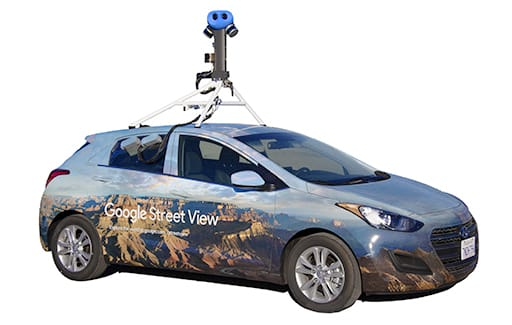
\includegraphics[width=\textwidth]{gsv-car}
    \\
    \cite[Quelle:][]{website:google-street-view:about}
  \end{center}
\end{wrapfigure}


Nachdem das Fahrzeug die Bilder aufgenommen hat, folgt die Nachbearbeitung. Hier
werden die einzelnen Bilder der Linsen in ein 360\degree\ Panorama zusammengestellt,
die Kennzeichen von anderen Fahrzeugen und die Gesichter von Personen verpixelt
und einige manuelle Nacharbeiten erledigt. Durch diesen Prozess dauert es von wenigen
Wochen bis zu mehreren Monaten bis die aufgenommenen Bilder in Goolge Street
View der Allgemeinheit verfügbar gemacht werden.

Neben den Kameras haben die Street View Fahrzeuge auch noch andere Sensoren:
beispielsweise ein genaues GPS-System, Messgeräte für Abstand, Tiefe und
Luftqualität. Zwischen 2008 und 2010 waren die Fahrzeuge auch mit einem WLAN
Scanner ausgestattet, das die Namen und MAC Addressen von Routern aufgezeichnet
hat, um die Positionierung in Android Smartphones zu verbessern.\footcite{website:trekview:gsv-sensors}

\subsection{Welche Daten kann man aus Google Street View erlangen}

In diesem Abschnitt wird gezeigt, wie die oben beschriebenen Daten von Google
und auch von allen anderen genutzt werden oder werden können, um einen Einblick
in die Möglichkeiten und die Implikationen für die Privatsphäre abzuschätzen

\subsubsection{WLAN Scanning}

Durch das WLAN Scanning hat Google folgende Daten erlangen können:

\begin{enumerate}
  \item Name und MAC Addresse des WLAN Routers oder Access Points \label{name-and-mac}
  \item Stärke des WLAN Signals an der jeweiligen Position \label{signal-strength}
  \item Netzwerkverkehr von ungesicherten WLAN Netzwerken \label{network-traffic}
\end{enumerate}

Durch die Punkte \ref{name-and-mac} und \label{signal-strength} ist es für
Google möglich, eine genauere Positionierung als GPS alleine anzubieten. Diese
Datensammlung ermöglicht Google eine Positionsbestimmung obwohl kein GPS Signal
erfangen werden kann; besonders in dichten Städten, in denen GPS Signale häufig
durch die hohen Häuser eingeschränkt sind und viele WLANs von den Häusern
ausgehen. Der Dienst der genauren Positionsbestimung findet anwendungs in Google
Smartphonebetriebssystem Android und der Google Maps App (unabhängig vom
Betriebssystem).

Im Gegensatz dazu steht der Punkt \ref{network-traffic}, der laut Google aus
Versehen gesammelt wurde. Die Daten würden von Google nicht genutzt werden.
Ebenso argumentiert Google, dass die Daten unvollständig sind, weil sich die
Fahrzeuge bewegen und der WLAN Channel fünfmal pro Sekunde gewechselt wird.\footcite{website:googleblog:wifi-data-collection}

Trotzdem wurde Google für diese Datensammlung sanktioniert. Die Daten mussten in
einigen Ländern gelöscht werden\footcite{website:isec:ireland-destroy-notice}, in
Deutschland gab es am 22.04.2013 wurde ein Bußgeld in Höhe von 145 000 EUR von dem
Hamburger Datenschutzbeauftragten Johannes Caspar verhängt\footcite{website:nwzonline:google-wifi-sanction}
und in den USA wurde vom Attorney General ein Bußgeld in Höhe von 7 Mio. USD verhängt.%\footnote{https://portal.ct.gov/AG/Press-Releases-Archived/2013-Press-Releases/Attorney-General-Announces-7-Million-Multistate-Settlement-With-Google-Over-Street-View-Collection-o}

\subsubsection{Fotos}

Die Daten aus dem WLAN Scanning sind nicht für alle verefügbar. Es werde auf der
Website und der mobilen App nur die 360\degree\ Panoramen bereitgestellt. Es ist
also interessant zu sehen, welche Daten man aus diesen Bildern extrahieren kann.

Die offentlichlichsten personenbezogenen Daten - Gesichter und Kennzeichen -
werden bereits automatisch verpixelt. Danach wird es durch Google Mitarbeiter
noch einmal validiert, dass diese Merkmale wirklich verpixelt wurden. Falls
dieser Prozess noch immer nicht alles verpixelt hat, bietet Google die
Möglichkeit ein Panorama zu melden, damit es noch einmal für eine manuelle
Sichtung und Nachbesserung markiert wird.

Es gibt aber durchaus andere Daten, die nicht für jeden ersichtlich sein sollen.
Bilder eines Einganges zu einer Basis der Britische Spezialeinheit SAS (Special
Air Services) haben dazu geführt, dass das MoD (Ministery of Defense) zur
Löschung der Bilder auffordert\footcite{website:bbc:herefordshire}. Ebenso ergab
sich ähnliches in den USA\footcite{website:reuters:pentagon-takedown-notice}.

Wissenschaftler\_innen nutzen Google Street View als Datengrundlage für eine
weitreichende Datenanalyse im Bereich Big Data und Machine Learning. Folgende
Themen und Werke werden als Beispiele näher beschrieben:

\begin{enumerate}
  \item Zur Planung von 5G Masten - \cite{Zhang_2020}\label{5g}
  \item Das Volumen an Fußgängern - \cite{YIN2015337}\label{pedestrian-volume}
  \item Die Demographie der Nachbarschaft - \cite{Gebru13108}\label{demographics}
  \item Die Wahrscheinlichkeit für einen Autounfall eines Bewohners - \cite{kita2019google}\label{car-accident}
  \item Die Gesundheit von Bewohnern einer bestimmten
  Nachbarschaft - \cite{8933431} und \cite{DBLP:journals/corr/abs-1905-06464}\label{health}
\end{enumerate}

In Arbeit \ref{5g} werden die Bilder von Google Street View genutzt, um
herauszufunden, wo sich Straßenbeleuchtungsmasten befinden. Es wird dadurch
möglich Masten für den neuen Funkstandard 5G zu planen, weil diese relativ
günstig an vorhandener Straßenbeleuchtung angebracht werden können.

Arbeit \ref{pedestrian-volume} misst das Volumen an Fußgängern, die zu der
Aufnahme der Google Street View Bilder draußen waren. Diese Daten können dann
genutzt werden, um zu urteilen, wie aktiv Menschen in einer Umgebung sind und
was Menschen dazu bringt mehr Zeit draußen zu verbringen. Weitere Informationen
über den Zusammenhang von Stadtbidl und physikalischer Aktivität findet man in
den Forschungsarbeiten vbon Li Yin an der State University of New York.

In Punkt \ref{demographics} wird gezeigt, dass die Google Street View Bilder
ebenso genutzt werden können, um Aussagen über die Nachbarschaft oder Region zu
treffen. In dieser Arbeit werden die fotografierten Autos (Marke, Modell und
Jahr) als Proxy für Demographie genutzt. Die Arbeit zeigt, dass wenn die Anzahl
der fahrenden Sedans höher ist als die Anzahl der Pickup Trucks, die Stadt
wahrscheinlich für die Demokraten stimmen wird. Eben falls konnten Einkommen,
Hautfarbe und Bildung aufgrund dieser Daten bestimmt werden.
% Die Arbeit von M. De Nadai et al. findet einen Zusammenhang zwischen
% der physikalischen Aktivität und der "Sicherheit" der Nachbarschaft. Die Daten
% über die "Sicherheit" kommen aus dem Place Pulse 2.0 Datensatz, in dem Menschen
% zwei Bilder von Häuserfronten und Straßen gezeigt wurde und diese urteilen
% mussten, welches Bild sicherer aussieht. Aus der Arbeit wird ähnlich wie bei
% \ref{pedestrian-volume} herausgearbeitet, welche Eigenschaften von Bildern
% besonders sicher aussehen.

Die Arbeit \ref{car-accident} beschreibt wie Bilder von Google Street View
besseren Aufschluss über die Wahrscheinlichkeit eines Autounfalls geben kann,
als andere Risikomodellen (beispielsweise basierend auf Alter, Postleitzahl),
die von Versicherungen genutzt werden. Diese Daten, argumentieren die Autoren,
können später auch von den Banken genutzt werden, da in anderen Arbeiten gezeigt
wurde, dass die Kreditwürdigkeit und Risikobewertung von Versicherungen
zusammenhängen\footcite{doi:10.1080/10920277.2016.1209118}.

Im Punkt \ref{health} ist zu sehen, dass die Bilder, die aus Google Street View
einzusehen sind, auch dafür genutzt werden können, um Aussagen über die
Gesundheit der Bewohner zu treffen. Solche Daten sind interessant für
Stadplaner, die überprüfen können, ob man etwas an der Umgebung ändern kann, was
die Bewohner anregt sich zu bewegen. Ebenfalls sind die Daten für
Krankenversicherungen interessant, um das Risiko von Krankheiten genauer abzuschätzen.

% - Daten, die GSV bereitstellt (Eventuell mehr recherchieren)
%   - https://arxiv.org/search/?query=google+street+view&searchtype=all&source=header
%   - http://eds.a.ebscohost.com/eds/results?vid=2&sid=a42b4726-42fd-40ba-b8c8-a49ef4322772%40sdc-v-sessmgr03&bquery=google+street+view&bdata=JmNsaTA9RlQxJmNsdjA9WSZsYW5nPWRlJnR5cGU9MCZzZWFyY2hNb2RlPUFuZCZzaXRlPWVkcy1saXZlJnNjb3BlPXNpdGU%3d

\subsection{Ein Pro und Contra zu Google Street View}

In diesem Unterkapitel werden die zuvor genannten Informationen
zusammengetragen, um Argumente für und gegen Google Street View zu bilden.

Grundsätzlich macht Google mit den Bildern nur einen Prozess einfacher: Anstatt
selbst die Straßen entlangzufahren, kann man einfach die Bilder von Google
Street View bekommen. Viele Forscher\_innen nutzen diese Daten, um einen Guten
Beitrag für die Menschheit zu bringen; es gibt dennoch Menschen mit
Motivationen, die diese Bilder für etwas Schlechtes nutzen.

% \begin{listing}
%   \item Soll Deutschland oder die EU von Google Stret View ausgeschlossen werden?
%   \item Soll nur die Neuaufnahme von Bildern verboten werden?
%   \item Dürfen die Google Street View Autos noch immer Daten für Google intern sammeln?
%   \item Soll Google Street View in Deutschland erweitert werden?
% \end{listing}


\subsubsection{Das Gute an Google Street View}

Wie in Unterkapitel \ref{street-view-detail} beschrieben werden Daten über
Luftqualität von Google gesammelt. Diese Daten können von Klimaforscher\_innen,
Stadtplanern und Regierungen genutzt werden, um den akteuellen Stand zum
Klimawandel zu überprüfen. Welche Maßnahmen sind effektiv? Wie lange dauert es,
um Verbessungen im CO2 Level zu messen? Welche Ursachen haben erhöhte Werte von
CO2 und Feinstaubpartikel?
Diese Daten helfen der Menschheit dabei, effektiv gegen den Klimawandel
vorzugehen und zukünftige Stadtprojekte nachhaltig zu planen.

Ebenso funktioniert auch die originalie Intention von Google Street View
wunderbar. Es ist für Autofahrer möglich die Route durch ein komplexes
Straßensystem schon vor Antriff der Reise zu planen. Sie können sich einige
markante Merkmale heraussuchen, die sie auf der Fahrt wiedererkennen. Dafür
müssen die Bilder von Google Street View aber aktuell sein. Leider ist
Deutschland dafür ein Schwarzes Loch; Es wurden nur knapp 20 Städte in Google
Street View aufgenommen und die Bilder stammen auf 2008 bis 2010.

Google zeigt durch eine Case Study, dass lokale Unternehmen von Google Street
View und Virtuellen Touren
profitieren\footcite{website:google:impact-for-loca-businesses}. Menschen gehen
lieber zu Lokationen, die einfach zu finden sind und von denen sie im vorhinein
sehen können, was sie erwartet. Das gilt für lokale Unternehmen als auch für den
Tourismus einer Region oder Landes. Eine weitere Einschränkung von Google Street
View würde dem Tourismus schaden, anders herum würde eine Ausweitung von Google
Street View sich positiv auf den Tourismus auswirken. Durch Google Street View
kann sich ein besserer Überblick über Sehenswürdigkeiten gemacht werden, als es
bei normalen Bildern ist. Dies führt dazu, dass man sich eher vorstellt einen
Urlaub dort zu verbringen. Es können auch potentielle Mieter oder Käufer vor dem
Kauf eines Hauses einschätzen, in welchen Zustand sich das Objekt befindet.


Zuletzt ist es möglich seine eigene Hausfront verpixeln zu lassen. Dieser
Opt-Out kann verhindern, dass bestimmte personenbezogene Daten ermittelt werden
können. Besonders die Kategorisierung des Hauses (Anzahl Fenster, Garage
vorhanden, Zustand des Hauses) oder des Autos (Marke, Modell) kann dadurch
verhindert werden. Genau diese Daten hatten es in den oben beschriebenen
Arbeiten ermöglicht Aussagen über Einkommen, Kreditwürdigkeit, Politische
Ausrichtung und anderen zu treffen.

\subsubsection{Das Schlechte an Google Street View}

Wie aus den vorangegangenen Arbeiten deutlich wurde, ist das automatische
Verpixeln häufig nicht gut genug, um alle Daten zu entfernen. Es bleiben noch
die Häuserfronten und Autos ersichtlich. Ebenso kann man Menschen an ihrem
Körperbau und Kleidung erkennen. Dies ist besonders ein Problem, wenn diese
Menschen gerade etwas machen, was in seinem\_ihrem Umfeld nicht positiv
wahrgenomen wird; etwa der Besuch eines Strip Clubs. Auch Googles Argument, dass
die Bilder von öffentlichen Straßen aufgenommen wurden, heißt nicht, dass diese
Bilder in der Art publiziert werde, wie sie es aktuell werden.

Sollte ein\_e Bewohner\_in den Opt-Out für seine\_ihre Hausfasade in Anspruch nehmen, kann es
in einer Art interpretiert werden, als hätte diese\_r etwa zu verstecken.
Versicherungen und Banken könnten einen Discount anbieten, wenn das Haus nicht
verpixelt ist (bzw. eine Penalty, wenn das Haus verpixelt ist).

Ein Argument, das sehr häufig genannt wird, ist dass es Einbrechern die Planung
eines Überfalls einfacher macht. Sie können sehen, welche Häuser isch lohnen zu
überfallen und nach potenziellen Eintrittspunkten ausschau halten. Dieses
Argument lässt sich aber dadurch entkräften, dass Einbrecher sowieso zum Raub
physikalisch anwesend sein müssen; ein vorheriges Scouten stellt daher kein
Problem dar, wenn ein Überfall geplant ist.

\subsection{Die Realität und Machbarkeit einer Einschränkung von Google Street View}

Eine sinnvolle Einschränkung von Google Street View wäre, dass Autos und
Menschen aus den Bildern retuschiert werden. Dadurch könnte der Zugriff auf
viele der Daten verhindert werden und Menschen würden nicht mehr in heiklen
Situationen verewigt werden. Leider ist dies ein großer Aufwand für Google, der
in den meisten Regionen nicht notwenig ist.

Das gleiche sieht das deutsche Recht: Jeder darf Bilder von öffentlichen Straßen
machen und veröffentlichen - auch Google. Nach dem KunstUrhG §23 dürfen Bilder
von Personen veröffentlich werden, wenn diese nur ein Beiwerk sind. Google
stellt sogar durch die Verpixelung sicher, dass Personen schwieriger bis gar
nicht mehr identifizierbar sind.

Ebenso sind Argumente, dass die Kamera in einer Höhe von 3 Metern montiert ist
und somit Einblick über Gartenzäune bekommen kann, vor Gericht entkräftet
worden\footnote{LG Berlin, Urteil vom 13.09.2010 - 37 O 363/10}.

Laut aktuellem Recht ist Google Street View vom Gesetz und Gericht bestätigt
worden. Es bleibt zuletzt die Frage, ob das Gesetz angepasst werden muss, um die
Freiheit von Personen und ihren Daten auch in der aktuellen digitalen Zeit zu
schützen. Diese Frage wird in Fazit noch einmal aufgegriffen.

\newpage
% Abschluss:
%   - Zusammenfassung der eingebrachten Perspektiven
%   - Fazit

\section{Fazit} \label{fazit}

Es gibt einige Vorteile durch Google Street View, doch ist mir meine
Privatsphäre wichtiger. Durch das Anfertigen dieser Arbeit wurde mir duetlich,
wie viele Informationen einfach nur durch die Bilder ersichtlich sind. Das
aktuelle Recht ist nicht darauf ausgelegt mit dem Internetgiganten Google
klarzukommen und deren Komglomerat aus Suchmaschine, Mail-Anbieter(GMail),
Werbeagentur (Google Ads und AdSense), Entertainment-Provider (YouTube),
Betriebssystementwickler (Android), Sicheheitstechnik-Vermarkter (Nest),
Internetanbieter (Google Fiber) und Datenhoarder in Form von Google
Street View.

Die Korrelationen, die Forscher\_innen alleine mit den Google Street View Bildern
anfertigen konnten, sind beängstigend. Es lässt sich nur vermuten, was Google
mit dem Verbund aller Daten erreicht. Diese Informationen können dann genutzt
werden, um Werbung noch besser und gezielter zu vermitteln oder sogar die politische
Meinung durch die Vorschläge bei YouTube zu prägen.

Das deutsche Recht ist mit einem solchen Anbieter überfordert und hält
fälschlicherweise an Gesetzen fest, die in einer Zeit geschrieben wurden, in
denen eine Massendatenerhebung und -haltung nicht möglich war.

Google Street View ist nur ein weiteres Produkt von Google, das zeigt, wie
durchsichtig der Mensch im digitalen Zeitalter geworden ist.


%-----------------------------------
% Anhang
%-----------------------------------
% \newpage
% \section*{Anhang} %Überschrift "Anhang", ohne Nummerierung
% \addcontentsline{toc}{section}{\langde{Anhang}\langen{Appendix}} %Den Anhang ohne Nummer zum Inhaltsverzeichnis hinzufügen
% \begin{appendices}
% \addtocontents{toc}{\protect\setcounter{tocdepth}{0}} %
% 	\renewcommand{\thesection}{\langde{Anhang}\langen{Appendix} \arabic{section}:}
% 	\renewcommand\thesubsection{\langde{Anhang}\langen{Appendix} \arabic{section}.\arabic{subsection}:}
% 	%\section{Beispielanhang}\label{Beispielanhang}
Dieser Abschnitt dient nur dazu zu demonstrieren, wie ein Anhang aufgebaut seien kann.
\subsection{Weitere Gliederungsebene}
Auch eine zweite Gliederungsebene ist möglich.
\section{Bilder}
Auch mit Bildern.
Diese tauchen nicht im Abbildungsverzeichnis auf.
\begin{figure}[H]
    \centering
    \caption[]{Beispielbild}
	\label{fig:Beispielbild}
    
\includegraphics[width=1\textwidth]{verzeichnisStruktur}
\end{figure}
% \end{appendices}
% \addtocontents{toc}{\protect\setcounter{tocdepth}{2}}

%-----------------------------------
% Literaturverzeichnis
%-----------------------------------
\newpage
%\addcontentsline{toc}{section}{Literatur}

% Die folgenden beiden Befehle würden ab dem Literaturverzeichnis wieder eine
% römische Seitennummerierung nutzen.
% Das ist nach dem Leitfaden nicht zu tun. Dort steht nur dass 'sämtliche
% Verzeichnisse VOR dem Textteil' römisch zu nummerieren sind. (vgl. S. 3)
%\pagenumbering{Roman} %Zähler wieder römisch ausgeben
%\setcounter{page}{4}  %Zähler manuell hochsetzen

% Ausgabe des Literaturverzeichnisses

% Keine Trennung der Werke im Literaturverzeichnis nach ihrer Art
% (Online/nicht-Online)
%\begin{RaggedRight}
%\printbibliography[heading=bibintoc,title={Literaturverzeichnis}]
%\end{RaggedRight}

% Alternative Darstellung, die laut Leitfaden genutzt werden sollte.
% Dazu die Zeilen auskommentieren und folgenden code verwenden:

% Literaturverzeichnis getrennt nach Nicht-Online-Werken und Online-Werken
% (Internetquellen).
% Die Option nottype=online nimmt alles, was kein Online-Werk ist.
% Die Option heading=bibintoc sorgt dafür, dass das Literaturverzeichnis im
% Inhaltsverzeichnis steht.
% Es ist übrigens auch möglich mehrere type- bzw. nottype-Optionen anzugeben, um
% noch weitere Arten von Zusammenfassungen eines Literaturverzeichnisse zu
% erzeugen.
% Beispiel: [type=book,type=article]
\printbibliography[nottype=online,heading=bibintoc,title={Literaturverzeichnis}]

% neue Seite für Internetquellen-Verzeichnis
\newpage

% Laut Leitfaden 2018, S. 14, Fussnote 44 stehen die Internetquellen NICHT im
% Inhaltsverzeichnis, sondern gehören zum Literaturverzeichnis.
% Die Option heading=bibintoc würde die Internetquelle als eigenen Eintrag im
% Inhaltsverzeicnis anzeigen.
%\printbibliography[type=online,heading=bibintoc,title={Internetquellen}]
\printbibliography[type=online,title={Internetquellen}]

\newpage
\pagenumbering{gobble} % Keine Seitenzahlen mehr

%-----------------------------------
% Ehrenwörtliche Erklärung
%-----------------------------------
\section*{
	\langde{Ehrenwörtliche Erklärung}
	\langen{Declaration in lieu of oath}}
\langde{Hiermit versichere ich, dass die vorliegende Arbeit von mir selbstständig und ohne unerlaubte Hilfe angefertigt worden ist, insbesondere dass ich alle Stellen, die wörtlich oder annähernd wörtlich aus Veröffentlichungen entnommen sind, durch Zitate als solche gekennzeichnet habe. Ich versichere auch, dass die von mir eingereichte schriftliche Version mit der digitalen Version übereinstimmt. Weiterhin erkläre ich, dass die Arbeit in gleicher oder ähnlicher Form noch keiner Prüfungsbehörde/Prüfungsstelle vorgelegen hat. Ich erkläre mich damit einverstanden, dass die Arbeit der Öffentlichkeit zugänglich gemacht wird. Ich erkläre mich damit einverstanden, dass die Digitalversion dieser Arbeit zwecks Plagiatsprüfung auf die Server externer Anbieter hochgeladen werden darf. Die Plagiatsprüfung stellt keine Zurverfügungstellung für die Öffentlichkeit dar.}
\langen{I hereby declare that I produced the submitted paper with no assistance from any other party and without the use of any unauthorized aids and, in particular, that I have marked as quotations all passages which are reproduced verbatim or near-verbatim from publications. Also, I declare that the submitted print version of this thesis is identical with its digital version. Further, I declare that this thesis has never been submitted before to any examination board in either its present form or in any other similar version. I herewith agree/disagree that this thesis may be published. I herewith consent that this thesis may be uploaded to the server of external contractors for the purpose of submitting it to the contractors’ plagiarism detection systems. Uploading this thesis for the purpose of submitting it to plagiarism detection systems is not a form of publication.}


\par\medskip
\par\medskip

\vspace{5cm}

\begin{table}[H]
	\centering
	\begin{tabular*}{\textwidth}{c @{\extracolsep{\fill}} ccccc}
		\myOrt, \the\day.\the\month.\the\year
		&
		% Hinterlege deine eingescannte Unterschrift im Verzeichnis /abbildungen und nenne sie unterschrift.png
		% Bilder mit transparentem Hintergrund können teils zu Problemen führen
		
\includegraphics[width=0.35\textwidth]{unterschrift}\vspace*{-0.35cm}
		\\
		\rule[0.5ex]{12em}{0.55pt} & \rule[0.5ex]{12em}{0.55pt} \\
		\langde{(Ort, Datum)}\langen{(Location, Date)} & \langde{(Eigenhändige Unterschrift)}\langen{(handwritten signature)}
		\\
	\end{tabular*} \\
\end{table}

\end{document}
